\chapter{Theory}\label{cha:theory}

\begin{comment}
The background theory depth and breadth depend on the depth needed to understand your project
in the different disciplines that your project crosses.
It is not a place to just write about everything you know that is vaguely connected to your project.
The theory is here to help the readers that do not know the theoretical basis of your work so that they
can gain sufficient understanding to understand your contributions --- and also for yourself to show that
you have understood the underlying theory and are aware of the methods used in the field.
In particular, the theory section provides
an opportunity to introduce terminology that can later be used without disturbing the text with a definition.
In some cases it will be more appropriate to have a separate section for different theories (or even separate chapters).
However, be careful so that you do not end up with too short sections.
Subsections may also be used to separate different background theories.

Be aware that ``background'' is a general term that refers to everything done by somebody else,
in contrast to the ``foreground'', which is your own work.
Hence there can (and will) be several background chapters, with the background theory being one of them
--- or several of them, since it thus is quite possible to split the background theory over more than one chapter,
e.g., by having a chapter introducing the theory directly needed for the research field in question and another
chapter discussing the machine learning theory, algorithms, tools, and evaluation methods commonly used in the field.
The related work chapter is thus also part of the background, while a chapter about data might be background
(if you only use somebody else datasets), but can also be part of the foreground (if you collect and/or annotate data
yourself, or if you process or clean the data in ways that can make it part of your own contribution).

It is ok to reuse material from other texts that you have written (e.g., the specialisation project), but if you do so, that must be clearly stated in the text, together with a description of how much of the text is new, old or rewritten/edited.
Such a statement about recycling of material in the Background Theory chapter can thus come here in the chapter introduction.

\section{Writing References in the Text}
\label{sec:writing_references}

When introducing techniques or results, always reference the source.
Be careful to reference the original contributor of a technique and not just someone who happens to use the technique.%
\footnote{But always make sure that you have read the work you are citing --- if not, cite someone who has!}
For results relevant to your work,
you would want to look particularly at newer results so that you have referenced the most up-to-date work in your area.
A common rule of thumb is to at least reference the first paper introducing the issue and the paper containing the latest / state-of-the-art
results. Additional papers making substantial contributions should also be referenced, as well as of course the ones you find most interesting.
Remember to use the right verb form depending on the number of authors.

If you do not have the source handy when writing, mark in the text that a reference is needed and add it later. \todo{add reference}
Web pages are not reliable sources --- they might be there one day and removed the next; and thus should be avoided, if possible.
A verbal discussion is not a source and should normally not be referenced
(though you can reference ``personal communication'', if there are no other options).
The bulk of citations in the report will appear in Chapter~\ref{cha:related_work}.
However, you will often need to introduce some terminology and key citations already in this chapter.

You can cite a paper in the following manner (and several other versions,
see the \verb!natbib! package documentation):

\section{The Reference List}
\label{sec:reference_list}

In general, make sure that the references that appear in your reference list can be easily located and identified by the reader.
So include not only authors and title, but year and place of publication, the full names of conferences and workshops,
page numbers in proceedings and collections, etc.
Hyperlinks or \acrfull{acr:doi} numbers are also nice to include.
Just as in the text itself, it is important to be consistent in the reference list, so include the same type of information for all references and write it in the same way.

% Check out the reference list at the end of this document for examples of how to write references in \BibTeX.
% Note a particular quirk: Many \BibTeX\ styles convert uppercase letters to lowercase, unless specifically told not to.
% You might thus need to ``protect'' characters that should not be converted, e.g., by writing \texttt{\{T\}witter} as in the \citet{FountaEA:18} reference.

% Also, keep in mind that `et' is a word in its own right (`and'), so there is no period after it (even though there is a period after `al.', which is short for `alia', meaning `others').
% Of course, when including such a reference in the text, the authors should be referred to in plural form. 
% So \citet{BenyonEA:13} state that life is good (not ``states'').

% Many sites, such as journals and \url{dblp.org} provide the matching \BibTeX\ entry for a reference. 
% However, you might still need to edit the entry in order to be consistent with the rest of your references.
% If you find references from sites such as \url{scholar.google.com} or \url{arXiv.org}, keep in mind that they often not are complete,
% so that you might need to add information to the entry (and probably edit it as well).

Some other good sites to find state-of-the-art work:
\begin{itemize}
    \item \url{paperswithcode.com}
    \item \url{nlpprogress.com}

\end{itemize}

\textit{Lorem ipsum dolor sit amet, consectetur adipiscing elit, sed do eiusmod tempor incididunt ut labore et dolore magna aliqua. Ut enim ad minim veniam, quis nostrud exercitation ullamco laboris nisi ut aliquip ex ea commodo consequat. Duis aute irure dolor in reprehenderit in voluptate velit esse cillum dolore eu fugiat nulla pariatur. Excepteur sint occaecat cupidatat non proident, sunt in culpa qui officia deserunt mollit anim id est laborum.}


\section{Introducing Figures}

\LaTeX is a bit tricky when it comes to the placement of ``flooting bodies'' such as figures and tables. It is often a good idea to let their code appear right before the header of the (sub)section in which they appear.
Note that you should anyhow always use an option for the placement (e.g., \verb|[t!]| to place it at the top of a page).

Do not just put the figure in and leave it to the reader to try to understand what the figure is.
The figure should be included to convey a message and you need to help the reader to understand the message
intended by explaining the figure in the text.
Hence \textbf{all} figures and tables should always be referenced in the text, using the \verb!\ref! command.
It is good practice to always combine it with a non-breakable space (\verb!~!) so that there will be no newline between the term referring to it and the reference, that is, using \verb!Figure~\ref{fig:BoxesAndArrowsAreNice}!.

Also, note that you can have a longer version of the figure (and table) caption attached to the actual figure,
while using the optional first argument to \verb!\caption! to include a shorter version in the list of figures (lof) or list of tables:
\begin{quote}
    \begin{verbatim}
\caption[Shorter lof text]{Longer text appearing under the figure}
\end{verbatim}
\end{quote}

\begin{figure}[t!]
    \centering
    \missingfigure{Here we will add an amazing figure explaining it all}
    \caption{A missing figure}
    \label{fig:AmazingFigure}
\end{figure}

In general it is good to add notes about things that you plan on writing later.
The \verb!todonotes! package is great for that kind of book-keeping, letting you write both shorter comments in the margin\todo{l8r dude} and longer comments inside the text, using the option \verb![inline]!.
\todo[inline]{There are always some more stuff that you will need to add at some later point.
    Be sure to at least make a note about it somewhere.}

\textit{Sed ut perspiciatis unde omnis iste natus error sit voluptatem accusantium doloremque laudantium, totam rem aperiam, eaque ipsa quae ab illo inventore veritatis et quasi architecto beatae vitae dicta sunt explicabo. Nemo enim ipsam voluptatem quia voluptas sit aspernatur aut odit aut fugit, sed quia consequuntur magni dolores eos qui ratione voluptatem sequi nesciunt. Neque porro quisquam est, qui dolorem ipsum quia dolor sit amet, consectetur, adipisci velit, sed quia non numquam eius modi tempora incidunt ut.}

\section{Introducing Tables in the Report}

\newcommand\emc{-~~~~}
\begin{table}[t!]
    \centering
    \caption[Example table]{Example table (F$_1$-scores); this table uses the optional shorter caption that will appear in the list of tables, so this long explanatory text will not appear in the list of tables and is only here in order to explain that to the reader.}
    \begin{tabular}{c|c|rrrrrr}
        \tabletop
        Langs                  & Source                                           & \multicolumn{1}{c}{Lang1} & \multicolumn{1}{c}{Lang2} & \multicolumn{1}{c}{Univ} & \multicolumn{1}{c}{NE} & \multicolumn{1}{c}{Mixed} & \multicolumn{1}{c}{Undef}
        \\ \tablemid
        \multirow{5}{*}{EN-HI} & FB+TW                                            & 54.22                     & 22.00                     & 19.70                    & 4.00                   & 0.05                      & 0.03                      \\
                               & FB                                               & 75.61                     & 4.17                      & 18.00                    & 2.19                   & 0.02                      & 0.01                      \\
                               & TW                                               & 22.24                     & 48.48                     & 22.42                    & 6.71                   & 0.08                      & 0.07                      \\
                               & Vyas                                             & 54.67                     & 45.27                     & 0.06                     & \emc                   & \emc                      & \emc                      \\
                               & FIRE                                             & 45.57                     & 39.87                     & 14.52                    & \emc                   & 0.04                      & \emc                      \\ \tablemid
        \multirow{2}{*}{EN-BN} & TW                                               & 55.00                     & 23.60                     & 19.04                    & 2.36                   & \emc                      & \emc                      \\
                               & FIRE                                             & 32.47                     & 67.53                     & \emc                     & \emc                   & \emc                      & \emc                      \\ \tablemid
        EN-GU                  & FIRE                                             & 5.01                      & \textbf{94.99}            & \emc                     & \emc                   & \emc                      & \emc                      \\
        \tablemid
        DU-TR                  & Nguyen                                           & 41.50                     & 36.98                     & 21.52                    & \emc                   & \emc                      & \emc                      \\ \tablemid

        EN-ES                  & \multirow{4}{*}{\rotatebox[origin=c]{90}{EMNLP}}
                               & 54.79                                            & 23.50                     & 19.35                     & 2.08                     & 0.04                   & 0.24                                                  \\
        EN-ZH                  &                                                  & 69.50                     & 13.95                     & 5.88                     & 10.60                  & 0.07                      & \emc                      \\
        EN-NE                  &                                                  & 31.14                     & 41.56                     & 24.41                    & 2.73                   & 0.08                      & 0.08                      \\
        AR-AR                  &                                                  & 66.32                     & 13.65                     & 7.29                     & 11.83                  & 0.01                      & 0.90                      \\ \tablebot
    \end{tabular}
    \label{tab:ExampleTable}
\end{table}

As you can see from Table~\ref{tab:ExampleTable}, tables are nice.
However, again, you need to discuss the contents of the table in the text.
You do not need to describe every entry, but draw the reader's attention to what is important in the table,
e.g., that 94.99 is an amazing F$_1$-score (and that probably something fishy happened there).
Use boldface, boxes, colours, arrows, etc. to mark the important parts of the table.

As can be seen in the example, elements in a table can sometimes benefit from being rotated (such as EMNLP in the `Source' column) or cover more than one row (EMNLP, as well as EN-HI and EN-BN in the `Langs' column) --- or more than one column, for that matter.
\end{comment}

\textit{Disclaimer: Parts from a paper written in the theory module "TDT13 - Advanced Text Analytics and Language Understanding" will be reused in the \nameref{cha:theory} chapter. This includes \autoref{subsec:attention-and-transformers} and \autoref{subsec:bert}.}

\vspace{12pt}

\Autochapterref{cha:theory} of this specialization project will lay the theoretical groundwork needed to understand the thesis. This includes central technologies and other considerations related to \glspl{acr:llm} and \glspl{acr:gis}. \autoref{fig:actor-map} shows an actor map which includes these \glspl{acr:llm} and their providers, as well as potential user groups, regulatory bodies that could affect adoption of \acrshort{acr:ai}-based technologies, and some relevant geospatial standards. Subsections \ref{sec:llms} through \ref{sec:ethical-and-privacy-concerns} will elaborate on each of the clusters of the actor map, starting with \glspl{acr:llm}.

\begin{figure}
    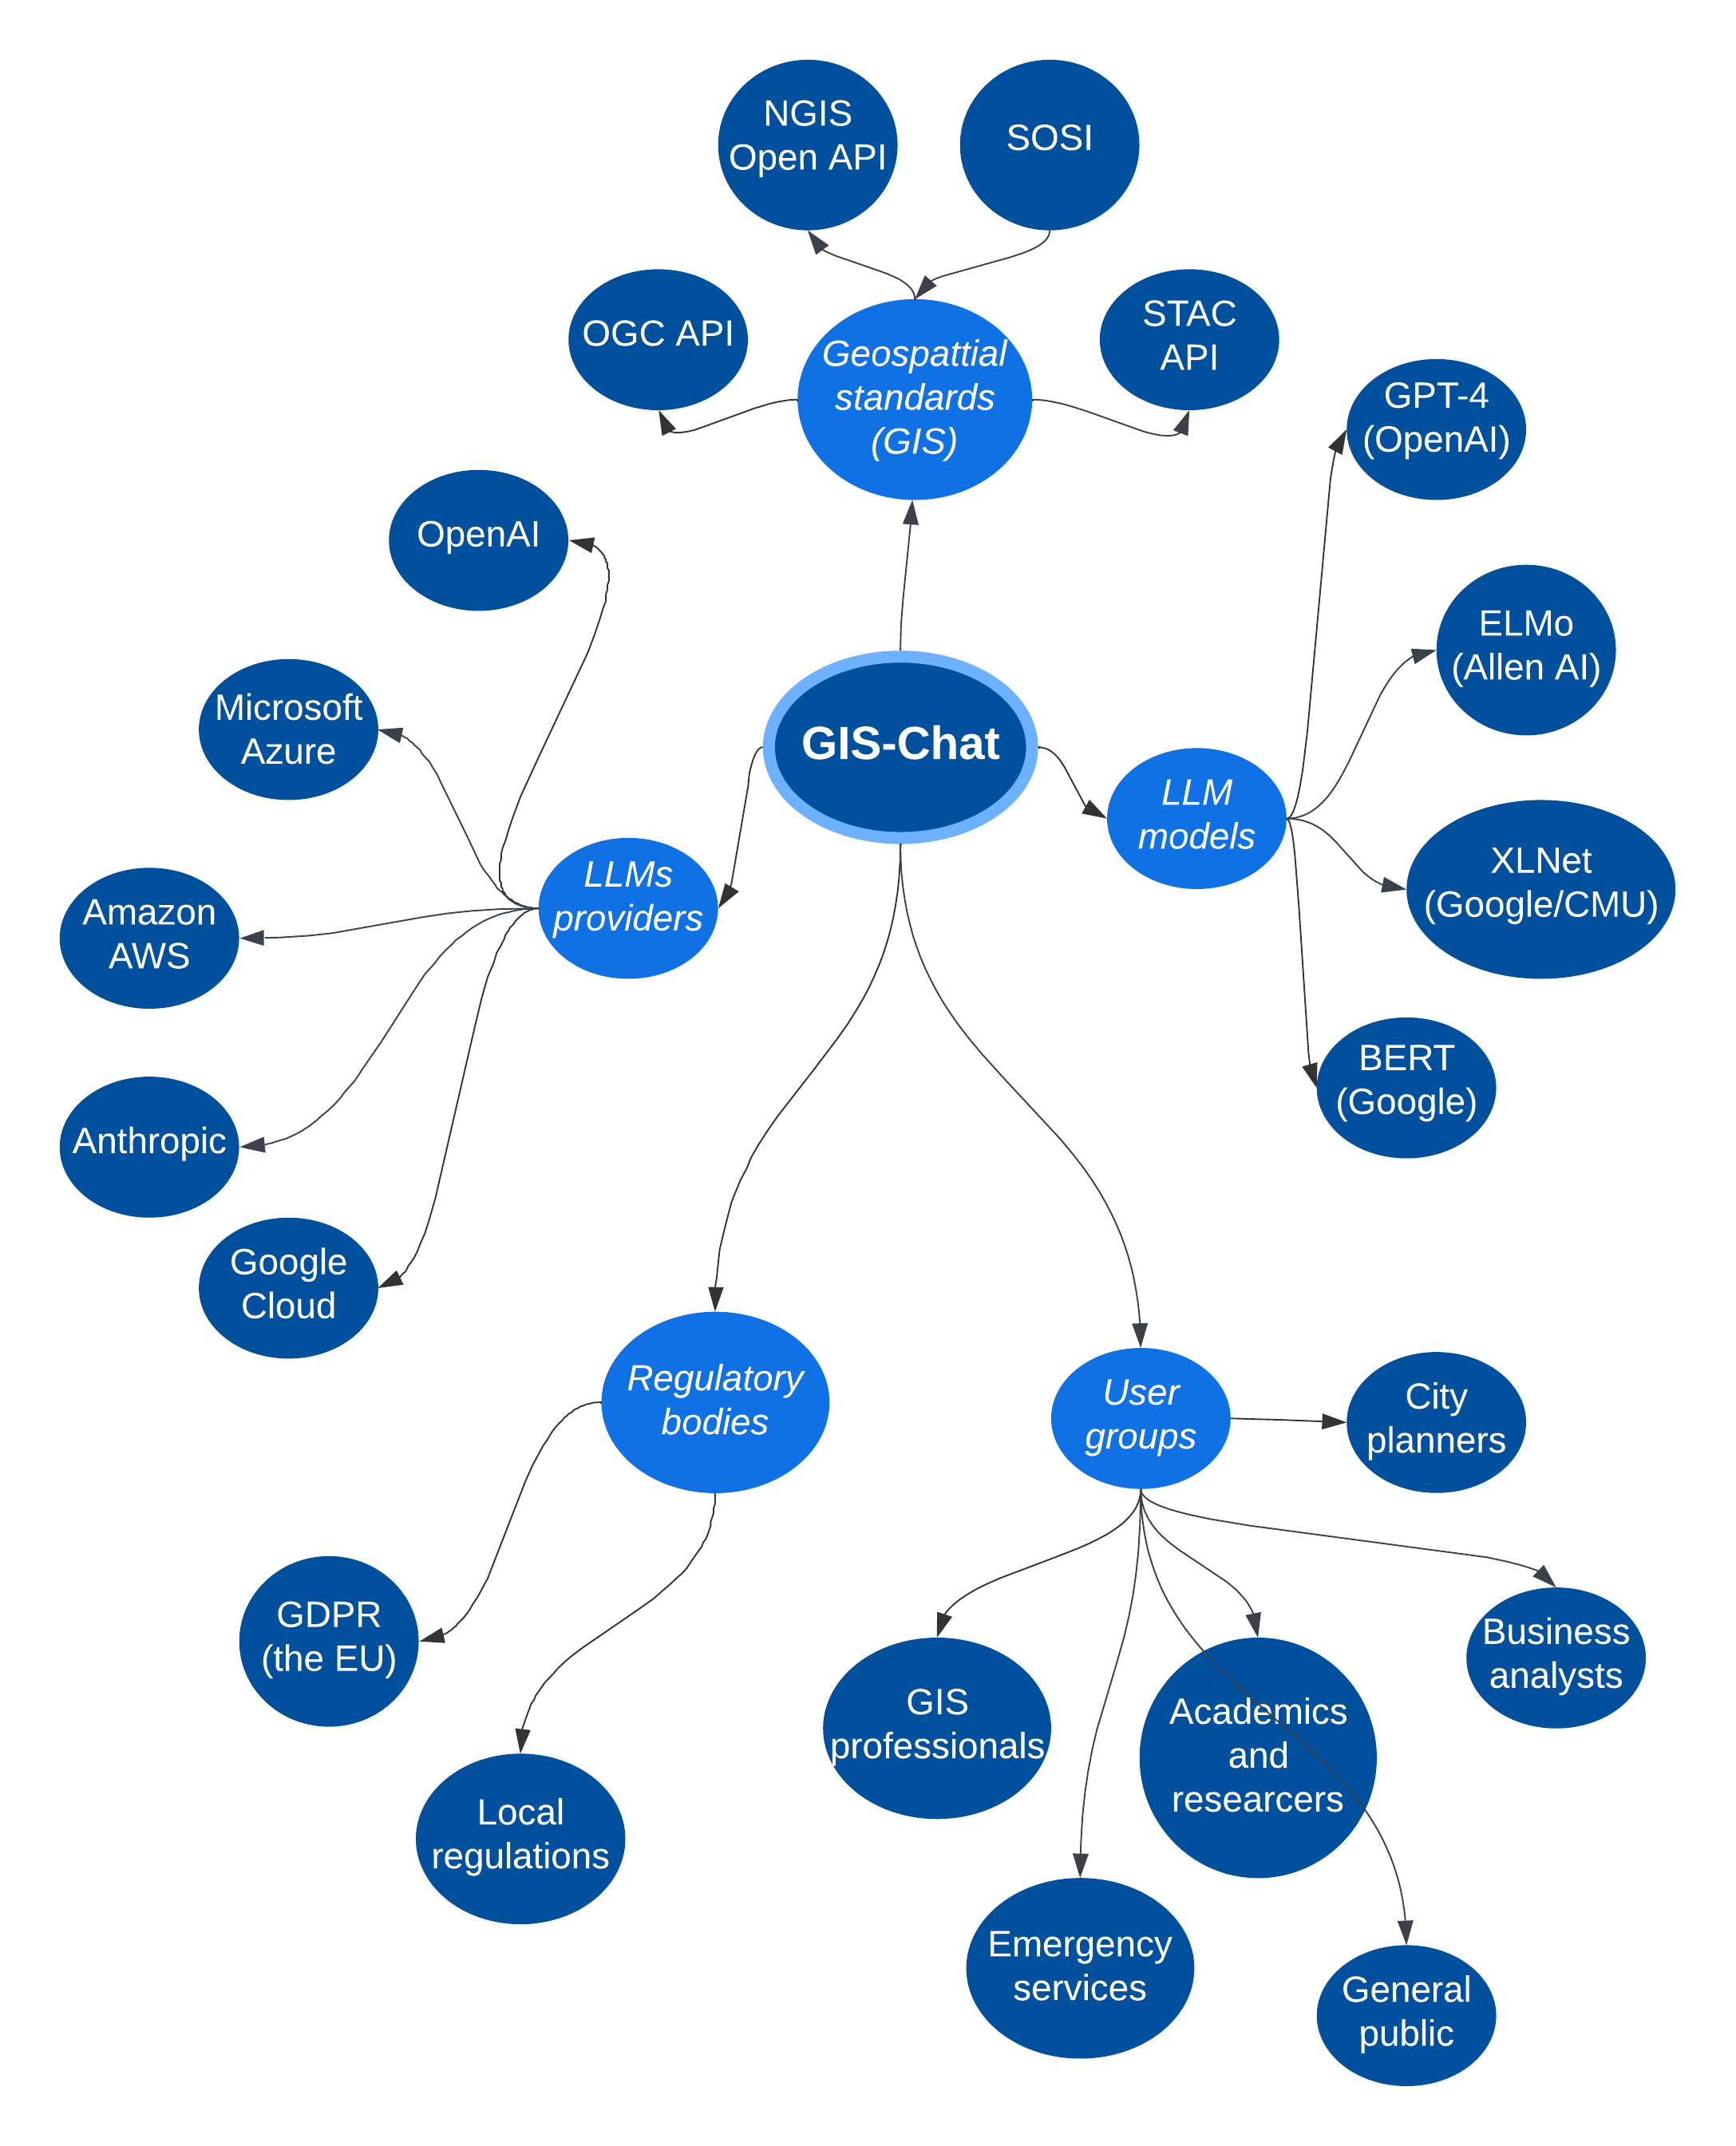
\includegraphics[width=\textwidth]{actor_map}
    \caption{Actor map for stakeholders, providers, and other groups and organizations that could have some relevance to an autonomous LLM-based GIS agent}
    \label{fig:actor-map}
\end{figure}

\section[Large Language Models]{\acrlongpl{acr:llm}}\label{sec:llms}

\acrfullpl{acr:llm} have proved proficient at \gls{acr:nlu} and \gls{acr:nlg}, which are both subfields of \gls{acr:nlp}. \autoref{fig:actor-map} includes six different \acrshortpl{acr:llm} that are all explained in the subsections below. All but the \acrshort{acr:bert} model are made with text generation in mind, with \acrshort{acr:bert} being more adapted for the task of predicting masked tokens, e.g. \enquote{I love going to the \texttt{[MASK]} during summer.}. \acrshort{acr:bert} is very efficient at \gls{acr:nlu}, and is applicable for a wide range of downstream tasks, one of which is discussed in \autoref{sec:gis-with-llms}. As mentioned, the other \acrshortpl{acr:llm} in \autoref{fig:actor-map} are geared towards text generation, with certain members of the \acrshort{acr:gpt} family and Google's Gemini having multimodal capabilities as well. As \autoref{subsec:social-media} will illustrate, these generative models---known for their great conversational abilities and extensive knowledge from pre-training on large corpora---have been found useful in \gls{acr:gis} analysis. The combination of conversational and visual skills---particularly in multimodal models---holds significant promise for \gls{acr:gis} analysis, where visual interpretation of maps is crucial.

This section will open with an explanation of the fundamental building block of modern \acrlongpl{acr:llm}: the Transformer. \Autosubsectionref{subsec:gpt} and \autoref{subsec:bert} will then discuss the two most famous families of \acrshortpl{acr:llm}, namely the \acrshort{acr:gpt}'s and the \acrshort{acr:bert}'s. \Autosubsectionref{subsec:gemini} will present the brand new multimodal Gemini model from Google, and \autoref{subsec:open-source-llms} will list various open-source alternatives.

\subsection{Attention and The Transformer Architecture}\label{subsec:attention-and-transformers}

\cite{vaswaniAttentionAllYou2017} managed to achieve new state-of-the-art results for machine translation tasks with their introduction of the Transformer architecture. The Transformer has later been proved effective for numerous downstream tasks, and for a variety of modalities. Titling their paper \citetitle{vaswaniAttentionAllYou2017}, \citeauthor{vaswaniAttentionAllYou2017} suggest that their attention-based architecture renders network architectures like \glspl{acr:rnn} redundant, due to its superior parallelization abilities and the shorter path between combinations of position input and output sequences, making it easier to learn long-range dependencies \citep[6]{vaswaniAttentionAllYou2017}.

The Transformer employs self-attention, which enables the model to draw connections between arbitrary parts of a given sequence, bypassing the long-range dependency issue commonly found with \glspl{acr:rnn}. An attention function maps a query and a set of key-value pairs to an output, calculating the compatibility between a query and a corresponding key \citep[3]{vaswaniAttentionAllYou2017}. Looking at \citeauthor{vaswaniAttentionAllYou2017}'s proposed attention function \eqref{eq:attention}, we observe that it takes the dot product between the query $Q$ and the keys $K$, where $Q$ is the token that we want to compare all the keys to. Keys similar to $Q$ will get a higher score, i.e., be \textit{more attended to}. These differences in attention are further emphasized by applying the softmax function. The final matrix multiplication with the values $V$, being the initial embeddings of the input tokens, will yield a new embedding in which all individual tokens have some context from all other tokens. We improve the attention mechanism by multiplying queries, keys, and values with weight matrices that are learned through backpropagation. Self-attention is a special kind of attention in which queries, keys, and values are all the same sequence.

\begin{equation}
    \text{Attention}(Q, K, V) = \text{softmax}\left(\frac{QK^T}{\sqrt{d_k}}\right)V
    \label{eq:attention}
\end{equation}

Attention blocks can be found in three places in the Transformer architecture \citep[5]{vaswaniAttentionAllYou2017} (I will use machine translation from Norwegian to German as an example):

\begin{enumerate}
    \item In the encoder block to perform self-attention on the input sequence (which is in Norwegian)
    \item In the decoder block to perform self-attention on the output sequence (which is in German)
    \item In the decoder block to perform cross-attention (also known as encoder-decoder attention) where each position in the decoder attends to all positions in the encoder
\end{enumerate}

The Transformer represented a breakthrough in the field of \gls{acr:nlp}, and is the fundamental building block of modern \glspl{acr:llm}, most famous of which are the \acrshort{acr:gpt}'s.

\subsection[The GPT Family]{The \acrshort{acr:gpt} Family}\label{subsec:gpt}

\gls{acr:gpt} is a type of \gls{acr:llm} that was introduced by OpenAI in 2018 \citep{radfordImprovingLanguageUnderstanding2018}. Specifically designed for text generation, a \acrshort{acr:gpt} is essentially a stack of Transformer \textit{decoders}, and demonstrates through its vast pre-training on unlabelled data that such unsupervised training can help a language model learn good representations, providing a significant performance boost while alleviating the dependence on supervised learning. While the original Transformer architecture as described by \cite{vaswaniAttentionAllYou2017} was intended for machine translation---thus having encoders to learn the representation of the origin language representation of a given input sequence and decoders to learn the representation in the target language and perform cross-attention between the two---the \acrshort{acr:gpt} is designed only to \textit{imitate} language. This is why there are no encoders to be found in the \acrshort{acr:gpt} architecture, only decoders. The model employs masked multi-head attention (running the input sequence through multiple attention heads in parallel), and is restricted to only see the last $k$ tokens---with $k$ being the size of the context window---and is tasked to predict the next one.

Training consists of two stages: unsupervised pre-training and supervised fine-tuning. The former is used to find a good initialization point, essentially teaching the model to imitate the corpora upon which it is trained. This results in a model that will ramble on uncontrollably, just trying to elaborate upon the input sequence it's given to the best of its knowledge. This will naturally produce undefined behaviour, and it is therefore necessary to fine-tune the model on target tasks in a supervised manner. \cite[4]{radfordImprovingLanguageUnderstanding2018} explain how the model can be fine-tuned directly on tasks like text classification, but how one for other tasks needs to convert structured inputs into ordered sequences because the pre-trained model was trained on contiguous sequences of text. In the case of ChatGPT, \citeauthor{openaiIntroducingChatGPT2022} used \gls{acr:rlhf} by employing a three-step strategy: first training using a supervised policy, then using trained reward models to rank alternative completions produced by ChatGPT models, before fine-tuning the model using \gls{acr:ppo}, which is a way of training \acrshort{acr:ai} policies. This pipeline is then performed for several iterations until the model produces the desired behaviour \citep{openaiIntroducingChatGPT2022}.

\subsection[The BERT Family]{The \acrshort{acr:bert} Family}\label{subsec:bert}

\gls{acr:bert}, introduced about four months after \cite{radfordImprovingLanguageUnderstanding2018} presented the \acrshort{acr:gpt} architecture, is a family of language models which was first introduced in 2018 and is designed to facilitate a wide range of downstream \gls{acr:nlp} tasks \citep[5]{devlinBERTPretrainingDeep2019}. The \acrshort{acr:bert} architecture consists of stacked bidirectional Transformer \textit{encoders}. This makes \acrshort{acr:bert} unsuitable for text generation, unlike the \textit{decoder}-based \acrshort{acr:gpt} architecture. However, the self-attention mechanism in the encoder---in which tokens can \textit{see} both past and future tokens---allows for training of deep bidirectional representations. The input sequence is first transformed into embeddings (vector representations). These per-token embeddings include information about the meaning of the word itself, the meaning of the sentence/segment it belongs to, and the token's position in the full input. These embeddings then pass through a stack of Transformer encoders (12 and 24 for \textbf{\acrshort{acr:bert}\textsubscript{BASE}} and \textbf{\acrshort{acr:bert}\textsubscript{LARGE}}, respectively), allowing the model to learn more complex patterns, and patterns of different granularities (token, sentence, document) \citep[5]{devlinBERTPretrainingDeep2019}.

The \acrshort{acr:bert} framework consists of two training steps: the pre-training and fine-tuning procedures. \acrshort{acr:bert} is pre-trained on two \gls{acr:nlp} tasks. One of these is \gls{acr:mlm}, in which 15\% of words are masked with the special \texttt{[MASK]} token and are left for the model to predict \citep[4]{devlinBERTPretrainingDeep2019}. The \gls{acr:mlm} task helps the model learn bidirectional representations. The second of these unsupervised tasks is \gls{acr:nsp}, where the special \texttt{[CLS]} token (found at the start of each tokenized sequence) is used to predict if a sentence \texttt{B} follows \texttt{A}. During this pre-training step, the input sequence looks like this:

$$
    \texttt{[CLS]} \text{ this is sentence A } \texttt{[SEP]} \text{ and this is sentence B } \texttt{[SEP]}
$$

\noindent The \texttt{[CLS]} token is used to label sentence B as either \texttt{IsNext} or \texttt{NotNext}.

\acrshort{acr:bert} is normally fine-tuned to specific downstream tasks by utilizing the \texttt{[CLS]} token representation after the last encoder layer, which captures an aggregated representation of the input sequence. This vector representation can then be used as input to a classification layer for tasks like multi-label classification and regression.

\subsection{Gemini}\label{subsec:gemini}

As of writing, Google's Gemini \citep{geminiteamGeminiFamilyHighly2023}, introduced on December 6th 2023, is the latest addition to the ever-growing pool of \acrlongpl{acr:llm}. Being fundamentally designed for multimodality, it is able to reason between text, images, video, audio, and code. It is being released in three different sizes: the Gemini Ultra, the Gemini Pro, and the Gemini Nano. The Gemini Ultra produces state-of-the-art performance on  out of 32 widely-used academic benchmarks, and performs worse than \citeauthor{openaiGPT4TechnicalReport2023}'s \acrshort{acr:gpt}-4 on only one benchmark, namely the HellaSwag benchmark for common-sense reasoning for everyday tasks. The Gemini Ultra outperforms \acrshort{acr:gpt}-4 on the \gls{acr:mmlu} benchmark, various reasoning benchmarks, and shows significant improvements in maths and code related benchmarks  \citep[7]{geminiteamGeminiFamilyHighly2023}. Gemini performs better than \citeauthor{openaiGPT4TechnicalReport2023}'s multimodal equivalent in \acrshort{acr:gpt}-4V on all benchmarks \citep[12]{geminiteamGeminiFamilyHighly2023}. Some of these benchmarks are discussed further in \autoref{subsec:benchmarks}.

Like the \acrshort{acr:gpt} architecture, Gemini is built on top of Transformer decoders. Gemini is trained to accommodate various modalities, supporting interleaved sequences of text, image, audio, and video as inputs \citep[3-4]{geminiteamGeminiFamilyHighly2023}. This highlights one of the greatest strengths of the Transformer architecture, namely that it can be adapted for multiple modalities. Commonly, multimodal \acrshort{acr:ai} architectures consist of an ensemble of models---one for each given modality---with different representations that can be difficult to combine. The Transformer solves this issue and provides a common architecture that can be trained end-to-end.

\subsection{Open-Source Alternatives}\label{subsec:open-source-llms}

Seeing as the state-of-the-art models of today, like \acrshort{acr:gpt}-4 and Gemini Ultra, are generally closed-source, it is important to note that there are viable open-source alternatives out there. This section lists the most prominent ones.

\subsubsection[LLaMA]{\acrshort{acr:llama}}

Perhaps the most famous family of open-source \acrshortpl{acr:llm} are Meta AI's \acrshort{acr:llama} (\acrlong{acr:llama}) models, with \acrshort{acr:llama} 2 being the latest addition \citep{touvronLlamaOpenFoundation2023a}. \acrshort{acr:llama} 2 is a powerful family of pre-trained and fine-tuned \acrshortpl{acr:llm} that outperformed open-source chat models on most benchmarks at its release. It also shows great results in terms of safety, even outperforming the closed-source ChatGPT-0301 model. The training process of \acrshortpl{acr:llama} is similar to that of the \acrshort{acr:gpt} model, with pre-training being performed using an optimized autoregressive transformer which is trained from a large corpus of unstructured data. \acrshort{acr:llama} is then fine-tuned using various alignment techniques, and the authors also share a new technique called Ghost Attention, which aims to control dialogue flow over multiple turns. \gls{acr:rlhf} and \gls{acr:ppo} are other important techniques used to get the desired behaviour out of the model.

Many flavours of \acrshort{acr:llama} have been trained. Most notably is Code \acrshort{acr:llama} 2 \citep{roziereCodeLlamaOpen2023}, a family of \acrshortpl{acr:llm} fine-tuned for code, scoring at 53\% and 55\% on the HumanEval and \gls{acr:mbpp} benchmarks, respectively. Vicuna-13B is another example of a \acrshort{acr:llama}-based model, and is fine-tuned on user-shared conversations collected from ShareGPT\footnote{\url{https://sharegpt.com/}}, a website where users can upload ChatGPT conversations. At its release in March 2023, it achieved more than 90\% quality of OpenAI's ChatGPT and Google's Bard, while also outperforming the original \acrshort{acr:llama} model.

\subsubsection{Mistral}

Mistral 7B \citep{mistralaiMistral7B2023} is another open-source \acrshort{acr:llm}, and is claimed by its creators at Mistral \acrshort{acr:ai} to be \enquote{the most powerful language model for its size to date}. Being a 7.3B parameter model, it is quite small compared to other models, such as the 1.76T parameter \acrshort{acr:gpt}-4 model. Mistral 7B outperforms the \acrshort{acr:llama} 2 13B on all benchmarks, and approaches Code \acrshort{acr:llama} 7B performance on code.

\subsubsection{Orca 2}

Orca 2 \citep{mitraOrcaTeachingSmall2023}---developed at Microsoft---is an open-source \acrshort{acr:llm} with exceptional step-by-step reasoning capabilities. It is based on \acrshort{acr:llama} 2 and is fine-tuned on curated training data from a more capable teacher model, like \acrshort{acr:gpt}-4. Evaluation results show that the Orca-2-13B model surpasses models of the same size, and that it is competitive with models 5-10x larger, exceeding the performance of \acrshort{acr:llama}-2-Chat70B and performing comparably to ChatGPT on reasoning tasks \citep[11-12]{mitraOrcaTeachingSmall2023}. It does have some limitations, most notably in terms of potential of misuse due to the lack of suitable safeguards like \gls{acr:rlhf} training \citep[21]{mitraOrcaTeachingSmall2023}.



\section[LLM providers]{\acrlong{acr:llm} Providers}\label{sec:llm-providers}

The \acrshort{acr:ai} community called Hugging Face\footnote{\url{https://huggingface.co/}} is the most widely used hub for open-source and open-science machine learning. It is used by both individual community members and large commercial actors like Google Cloud and Meta \acrshort{acr:ai} as a way of contributing to the world open-source \acrshort{acr:ai}. Hugging Face's \texttt{transformers}\footnote{\url{https://github.com/huggingface/transformers}} Python library provides an interface with their hub, which at the time of writing has 177k stars on GitHub.

OpenAI is one of the leading providers of \acrshortpl{acr:llm}, most prominently through their \acrshort{acr:gpt} series. While originally founded as an open-source company, their models are now closed-source and their \acrshort{acr:gpt} \acrshortpl{acr:api} are paid services. It should be noted, however, that they still are great contributors to open-source \acrshort{acr:ai}, having uploaded a range of speech detection and diffusion models to Hugging Face.

Microsoft Azure---the main partner of OpenAI---provides \acrshortpl{acr:api} for OpenAI's language models including the \acrshort{acr:gpt}-4, \acrshort{acr:gpt}-3.5-Turbo, and Embeddings model series. Unlike OpenAI's own \acrshortpl{acr:api}, Microsoft Azure also offers private networking, regional availability, and responsible \acrshort{acr:ai} content filtering.\footnote{\url{https://learn.microsoft.com/en-us/azure/ai-services/openai/overview?source=recommendations}} Also, by using Microsoft Azure's \acrshort{acr:api}, \acrshort{acr:llm} inputs and outputs are unavailable to OpenAI, which is not the case otherwise.\footnote{\url{https://learn.microsoft.com/en-us/legal/cognitive-services/openai/data-privacy}}

\cite{clearyLatencyBenchmarksComparisons2023} did benchmarking of different \acrshortpl{acr:llm} on different providers. Important takeaways were that \acrshort{acr:gpt}-4 is about 6.3 times slower than \acrshort{acr:gpt}-3.5-Instruct, and that Microsoft Azure has far lower latency in most cases for inference on \acrshort{acr:gpt} models compared to OpenAI's own \acrshortpl{acr:api}. Such considerations are important when addressing usability of \acrshort{acr:llm}-based applications, balancing accuracy against speed and cost.

Aforementioned Google Cloud is another large \acrshort{acr:llm} provider. They provide a wide range of services, among these the Vertex \acrshort{acr:ai} platform.\footnote{\url{https://cloud.google.com/vertex-ai/}} Vertex \acrshort{acr:ai} provides \acrshort{acr:api} access to foundational models through their Model Garden platform which supports first-party, open-source, and third-party models. Vertex \acrshort{acr:ai} also provides experimental prompt design and fine-tuning services. Vertex \acrshort{acr:ai} is a paid service.

Anthropic\footnote{\url{https://www.anthropic.com/}} is another closed-source \acrshort{acr:llm} provider that has grown rapidly in size since their launch in 2021. They focus on creating safer, steerable, and more reliable models. Their flagship model is Claude 2.1, which has a large context window of 200,000 tokens, enabling users to upload large technical documentation that the model can keep in its memory when generating responses. Anthropic lists complex reasoning, creativity, and coding as Claude's major strengths.

There are numerous open-source alternatives to these closed-source resources. Using free open-source alternatives where possible is a good option to reduce cost. Meta \acrshort{acr:ai}\footnote{\url{https://ai.meta.com/}} is a big contributor to open-source \acrshort{acr:ai}, most famously through Pytorch---a popular deep learning framework---and their LLaMA models (see \autoref{subsec:open-source-llms}). Eleuther \acrshort{acr:ai}\footnote{\url{https://www.eleuther.ai/}} is an open-source centred company with aim to \enquote{increase transparency and reduce potential harms from emerging \acrshort{acr:ai} technologies}. As such, they have released a range of trained \acrshortpl{acr:llm} along with the codebases used to train these. Perhaps most famous is their \acrshort{acr:gpt}-J model, which is an autoregressive model in the style of \acrshort{acr:gpt}-3, aimed at the English language.

\section{Geospatial Standards}\label{sec:geospatial-standards}

It is important for \acrshort{acr:gis} applications of any kind to support modern geospatial standards. \Autosubsectionref{subsec:standardization-international} will offer a brief overview of the standardization efforts on the international stage, while \autoref{subsec:standardization-norway} will similarly cover these efforts within the context of Norway.

\subsection{International Standardization Work}\label{subsec:standardization-international}

International geospatial standardization involves the global collaboration and development of uniform standards and protocols for geospatial data and technologies. The \acrshort{acr:ogc} standards and the \acrshort{acr:stac} \acrshort{acr:api} standard are examples of such work.

\subsubsection[OGC Standards]{\acrshort{acr:ogc} Api Standard}\label{subsubsec:ogc}

The \gls{acr:ogc} \acrshort{acr:api} standards serve as the glue in the field of \gls{acr:gis}, paving the way for interoperability and data exchange between diverse systems. Supporting multiple data formats including \acrshort{acr:json}, \acrshort{acr:gml}, and \acrshort{acr:html}, the \gls{acr:ogc} \acrshort{acr:api} standard provides a modular architecture consisting of a core specification and various extensions. According to their webpages, they provide 80 different standards, each for a specific geospatial purpose. Notable examples are 3D Tiles, CityGML, GeoTiff, and \acrshort{acr:ogc} \acrshort{acr:api} - Features \citep{ogcOGCStandards2023}. The \acrshort{acr:ogc} \acrshort{acr:api} standards function as modern replacements to older standards like \acrshort{acr:wms} and \acrshort{acr:wfs}, and presents a more adaptable framework for spatial data operations, facilitating innovation in the \acrshort{acr:gis} domain.

\subsubsection[STAC Api Standard]{\acrshort{acr:stac} Api Standard}\label{subsubsec:stac}

The \gls{acr:stac} \acrshort{acr:api} is a standardized way to expose collections of spatial temporal data for online search and discovery. Built upon a \acrshort{acr:json} core, it aims to be a uniform and flexible environment from which developers can customize the API infrastructure to their domain. \acrshort{acr:stac} is closely related to \acrshort{acr:ogc}, and \acrshort{acr:ogc} board member Chris Holmes said the following in a blog post: \enquote{The \acrshort{acr:stac} \acrshort{acr:api} implements and extends the \gls{acr:ogc} \acrshort{acr:api} - Features standard, and our shared goal is for \gls{acr:stac} \acrshort{acr:api} to become a full \gls{acr:ogc} standard.} \citep{holmesSpatioTemporalAssetCatalogs2021}. \gls{acr:stac} \acrshort{acr:api} provides a powerful query language that allows users to search by various parameters like time, location, and keywords, making it widely applicable. The \acrshort{acr:stac} community has also defined specifications in order remove the complexity associated with having to create unique pipelines when consuming different spatio-temporal collections. The significance of the \gls{acr:stac} \acrshort{acr:api} lies in its ability to democratize access to large volumes of geospatial data. By offering a common standard for data cataloguing and discovery, it reduces the barriers that often exist due to incompatible data formats. Developers or \acrshort{acr:gis} professionals can take advantage of this through built-in tooling in QGIS---a desktop \gls{acr:gis} for viewing, editing, and analysing spatial data---or through third-party packages in the Python and R programming languages. The API is also accessible through the command line interface when using \acrshort{acr:gdal} \citep{STACTutorials}.

\subsection{Norwegian Standardization Work}\label{subsec:standardization-norway}

Geospatial standardization work has been on the agenda of Norwegian governing powers for decades and have materialized in frameworks/collaborations like \nameref{subsubsec:geovekst} and \nameref{subsubsec:norge-digitalt}, as wells as the \nameref{subsubsec:sosi} file format. This standardization work will be the topic of this section.

\subsubsection[SOSI]{\acrshort{acr:sosi}}\label{subsubsec:sosi}

\gls{acr:sosi} is a Norwegian file format for storing and exchanging geospatial data. It was first introduced in 1987 and has since approached international standards, with the most important arenas being \acrshort{acr:iso}/\acrshort{acr:tc} 211 and \gls{acr:ogc} \citep{mardalNasjonalStrategiVidereutvikling2015}. \gls{acr:sosi} is the adopted Norwegian standard for creating and delivering digital geographic data, and is administered by the Norwegian Mapping Authority \citep{maehlumSOSI2023}.


In a \gls{acr:sosi} dataset, terrain points, lines, and polygons are represented by their coordinates and classified into various object types according to the \gls{acr:sosi} object catalogue standard. However, there are few GIS systems that can read \gls{acr:sosi} data directly, so data in \gls{acr:sosi} format usually needs to be converted into more \gls{acr:gis}-friendly data formats \citep{maehlumSOSI2023}.

\subsubsection{Geovekst}\label{subsubsec:geovekst}

Geovekst is a Norwegian initiative that aims for collaborative collection, distribution, management, and maintenance of geospatial information. It was established in 1992, and is a partnership between national, regional, and local government bodies, as well as several private companies.\footnote{\url{https://www.kartverket.no/geodataarbeid/geovekst}} The primary goal associated with Geovekst is to \enquote{collaborate to secure updated Geovekst data to help solve parts of the parties' societal missions} \citep[5]{thenorwegianmappingauthorityHandbokGeovekstsamarbeidet2023}. The objective of the collaboration is to ensure that geographical data is collected \textit{once}, conforming  to \textit{one} standard, maintained in \textit{one} place, and used by \textit{many}. Responsibilities and costs are shared among the parties of the collaboration.

The most important contribution of Geovekst is \gls{acr:fkb}, a series of very detailed Norwegian mapping datasets, serving as rich resources for both public and private sectors. The datasets are obtained through a variety of data sources, including aerial photographs, laser scans, and manual mapping. Geovekst also provides airborne surveys in emergency situations, when the speed of surveying is important.\footnote{\url{https://www.kartverket.no/geodataarbeid/geovekst/datafangst-i-krise}}

\subsubsection[The National Spatial Data Infrastructure]{The \acrlong{acr:nsdi}}\label{subsubsec:norge-digitalt}

Established in 2005, the \gls{acr:nsdi} is a more recent framework compared to Geovekst, and is more often referred to by its Norwegian name: \textit{Norge Digitalt}. The \gls{acr:nsdi} involves governmental bodies (national, regional, and municipal), but also educational and research institutions and companies with responsibilities on a nation-wide scale; examples include Telenor and local and regional energy companies \citep[6]{norgedigitaltGenerelleVilkarNorge2023}. The \gls{acr:nsdi} infrastructure is the sum of common standards and rules, geographical data and services related to these, in addition to tools and deals. It aims to coordinate geospatial activities in Norway, making it easier to discover, access, and use spatial data. The framework is coordinated by the Norwegian Mapping Society \citep{norgedigitaltGenerelleVilkarNorge2023}.



\section{User Groups}\label{sec:user-groups}

\begin{table}[ht]
    \centering
    \begin{tabular}{l|c}
        \toprule
        \textbf{Category}                    & \textbf{Percentage} \\
        \midrule
        Task oriented                        & 23.1\%              \\
        Informational                        & 20.2\%              \\
        Social                               & 16.2\%              \\
        Personal advice and self-improvement & 13.1\%              \\
        \bottomrule
    \end{tabular}
    \caption{Distribution of query categories \citep{kumarWhatArePeople2023a}}
    \label{tbl:query-category-distribution}
\end{table}

There are several user groups that could take advantage of an \acrshort{acr:llm}-based agent with extensive geographic and \acrshort{acr:gis} knowledge. Queries to such an agent could span from simple retrieval questions like \enquote{How many people live in Trondheim?} and \enquote{What is Sweden's third largest city?}, to more complicated questions that require problem-solving abilities and reasoning. While it is difficult to obtain good datasets of common queries, \cite{kumarWhatArePeople2023a}---creator of the chatbot app Pocket AI\footnote{\url{https://github.com/varunon9/pocket-ai}}---shared a dataset of \textasciitilde 13k user queries from his app along with classifications of these. Salient categories are listed in \autoref{tbl:query-category-distribution}. The main takeaway from these numbers is that the main motivation for use is productivity.

\begin{table}[ht]
    \centering
    \begin{tabular}[t]{l|c}
        \toprule
        \textbf{Category}              & \% \textbf{(n)} \\
        \midrule
        Productivity                   & 55\% (109)      \\
        Novelty                        & 51\% (101)      \\
        Fun and amusement              & 20\% (41)       \\
        Creative work                  & 18\% (34)       \\
        Social interaction and support & 9\% (18)        \\
        Other                          & 7\% (15)        \\
        \bottomrule
    \end{tabular}
    \caption{Categories and frequency of ChatGPT usage \citep[16-17]{skjuveWhyPeopleUse2023}}
    \label{tbl:chatgpt-motivation-survey-restuls}
\end{table}

This aligns with the results of \cite{skjuveWhyPeopleUse2023} from their questionnaire-based study performed in late January 2023, about two months after the release of ChatGPT. The goal with the study was to figure out why people use ChatGPT. They found that most participants (55\%) are motivated by productivity, specifically applying it for routine tasks, information retrieval, text generation and writing support, and software development \citep[17-21]{skjuveWhyPeopleUse2023}. \autoref{tbl:chatgpt-motivation-survey-restuls} shows all categories and their frequencies. There were 197 samples in total, and more than one category could be  assigned to each sample. It is worth noting that the study is likely to have included early adopters, and might therefore make the results less representative for the time at which this report is written (\today), now that use patterns have become more established \citep[37]{skjuveWhyPeopleUse2023}.

The main reason people use conversational \acrshort{acr:ai} is clearly to increase productivity, whether in a professional, academic, or personal context. 67 out of the 197 participants in \cite[18]{skjuveWhyPeopleUse2023} highlighted ChatGPT's ability to understand complex queries and that it is \enquote{efficient in alleviating the need to experiment with different phrasings of the query}, as is often needed when 'Googling' for an answer to a specific question. The ease of information retrieval, along with it's problem-solving abilities \citep[20]{skjuveWhyPeopleUse2023}, could also make conversational \acrshortpl{acr:ai} highly relevant for \acrshort{acr:gis}-related purposes.

One could imagine a range of potential user groups that could benefit from such an artificial, and spatially aware, companion. Some suggested user groups are presented in \autoref{fig:actor-map}. Perhaps the most obvious one is that of the \acrshort{acr:gis} professionals. While an \acrshort{acr:ai}-based \acrshort{acr:gis} agent more capable than the average \acrshort{acr:gis} professional is currently far from becoming a reality, such an agent could help suggest strategies of solving a particular problem using the input data available and a good user prompt, or it could help solve mundane tasks in an automated way in order to allow \acrshort{acr:gis} professionals to allocate more time to creative and complex tasks.

Closely related to \acrshort{acr:gis} professionals are the city planners. Though often less knowledgeable in the field of \acrshort{acr:gis}, they are increasingly dependent upon geospatial analyses in order to make informed decisions. Having an easy-to-use \acrshort{acr:gis} agent ready at any moment could prove both time- and cost-saving. The same goes for business analysts and people involved in academia. The \textit{time} variable is especially important to the emergency services. At the impact of a natural disaster like a flood or forest fire, geospatial analysis could prove lifesaving. Having powerful geospatial knowledge even in the absence of a \acrshort{acr:gis} professional is therefore important in order to focus resources to areas where the situation is most pressing.

An \acrshort{acr:llm}-based agent with geospatial awareness could also be useful to the general public: one may want to find suitable biking routes or good hills for interval running, or to identify areas prone to flooding when buying a house. Most people do not possess the knowledge or time to perform such analyses themselves, so an automated \acrshort{acr:ai}-based agent could prove useful for such use cases.



\section{Ethical and Privacy Concerns}\label{sec:ethical-and-privacy-concerns}

Although an \acrshort{acr:llm}-based \acrshort{acr:gis} agent could prove powerful, there are some ethical pitfalls in terms of regulations and privacy concerns that need consideration. If such an agent is to make decision on behalf of humans it is important that one can hold someone accountable in the case that something goes wrong. If an \acrshort{acr:ai}-based agent is tasked to lead firefighters to the tactically optimal locations in order to quench a fire, but  instead misleads them and traps them inside the fire, who is then to blame? \cite{sparrowKillerRobots2007} provides an interesting angle on such issues, though in his essay related the role of artificially intelligent robots in modern warfare.

Furthermore, it is vital to ensure that the \acrshort{acr:ai} agent is not utilized for immoral purposes, like finding the optimal location in which to dissolve poison into people's drinking water to maximize the number of people killed. Work has been done with newer \acrshortpl{acr:llm} to prevent them from producing dangerous, misinformed, or toxic text---this issue is widely discussed in the technical report of the latest \acrshort{acr:gpt} model \citep[11-14]{openaiGPT4TechnicalReport2023}---but there have been cases where these issues haven't been considered well enough.\footnote{The \acrshort{acr:llama}-based Alpaca model, developed at Stanford University, was taken offline after being shown to produce misinformation, toxic text: \url{https://www.theregister.com/2023/03/21/stanford_ai_alpaca_taken_offline/}}

The \gls{acr:gdpr} entered into applicability in the European Union on 25th of May 2018, and although not a member of the European Union, Norway incorporated the \gls{acr:gdpr} in July the same year due to its membership of the European Economic Area. The \gls{acr:gdpr} imposes stricter regulations about data privacy, meaning people have more control over their personal data, and that businesses get a level playing field in terms of what customer information is available \citep{datatilsynetGeneralDataProtection}. With data privacy arguably being more relevant than ever, we must make certain that \acrshort{acr:llm}-based \acrshort{acr:gis} agents are unable to access and spread information of private or sensitive character, even if such information has become publicly available by accident---as was the case when the Norwegian Broadcasting Corporation (NRK) was able to (legally) obtain accuracy geolocations of central people in the Norwegian army from a commercial London-based company\footnote{Link to news article in Norwegian: \url{https://www.nrk.no/norge/xl/norske-offiserer-og-soldater-avslort-av-mobilen-1.14890424}}.

\glsresetall